\documentclass[12pt,a4paper]{article}
\usepackage[utf8]{vietnam}
\usepackage{amsmath,amssymb}
\usepackage{tabularx}
\usepackage{tikz}
\usetikzlibrary{calc,angles,quotes,arrows.meta,patterns}
\usepackage{xcolor}
\usepackage{enumitem}
\usepackage{fancyhdr}
\usepackage{graphicx}
\usepackage[top=1.2cm, bottom=1.2cm, left=1.5cm, right=1.5cm]{geometry}
\usepackage[loigiai]{ex_test}
\SAOPTN{widthSA=2.6,heightSA=0.62}

\setlength{\headheight}{15pt}
\setlength{\parskip}{0pt}

\pagestyle{fancy}
\fancyhf{}
\rhead{\textit{Môn Toán 6 -- Hướng dẫn giải Đề số 14}}
\lhead{\textit{Bộ đề ôn tập Giữa học kì I}}
\cfoot{\thepage}

\begin{document}

\begin{center}
  \textbf{\Large HƯỚNG DẪN GIẢI CHI TIẾT VÀ BẢNG ĐÁP ÁN}\\
  \textbf{\large ĐỀ ÔN TẬP GIỮA HỌC KỲ I -- ĐỀ SỐ 14}\\
  \textit{Môn: Toán 6 -- Năm học 2026 -- 2027}
\end{center}
\vspace{2mm}

% --- BẢNG ĐÁP ÁN TRẮC NGHIỆM TÓM TẮT ---
\noindent\textbf{\large A. BẢNG ĐÁP ÁN TRẮC NGHIỆM TỔNG HỢP}
\vspace{1.5mm}

\noindent\textbf{1. Phần I (Mỗi câu trả lời đúng được 0,25 điểm):}
\begin{center}
\begin{tabular}{|c|c|c|c|c|c|c|c|c|c|c|c|c|}
\hline
\textbf{Câu} & \textbf{1} & \textbf{2} & \textbf{3} & \textbf{4} & \textbf{5} & \textbf{6} & \textbf{7} & \textbf{8} & \textbf{9} & \textbf{10} & \textbf{11} & \textbf{12} \\
\hline
\textbf{Đ/A} & \textbf{A} & \textbf{B} & \textbf{C} & \textbf{A} & \textbf{B} & \textbf{A} & \textbf{C} & \textbf{C} & \textbf{D} & \textbf{B} & \textbf{B} & \textbf{A} \\
\hline
\end{tabular}
\end{center}
\vspace{1mm}

\noindent\textbf{2. Phần II (Đúng 1 ý: 0,1đ; 2 ý: 0,25đ; 3 ý: 0,5đ; 4 ý: 1,0đ):}
\begin{center}
\begin{tabular}{|c|c|c|c|c||c|c|c|c|c|}
\hline
\textbf{Câu} & \textbf{a)} & \textbf{b)} & \textbf{c)} & \textbf{d)} & \textbf{Câu} & \textbf{a)} & \textbf{b)} & \textbf{c)} & \textbf{d)} \\
\hline
\textbf{Câu 1} & \textbf{Đ} & \textbf{Đ} & \textbf{Đ} & \textbf{S} & \textbf{Câu 2} & \textbf{Đ} & \textbf{Đ} & \textbf{S} & \textbf{Đ} \\
\hline
\end{tabular}
\end{center}
\vspace{1mm}

\noindent\textbf{3. Phần III (Mỗi câu trả lời đúng được 1,0 điểm):}
\begin{center}
\begin{tabular}{|c|c|c|}
\hline
\textbf{Câu} & \textbf{Câu 1} & \textbf{Câu 2} \\
\hline
\textbf{Đáp án} & \textbf{20} & \textbf{15} \\
\hline
\end{tabular}
\end{center}
\vspace{3mm}

% --- B. LỜI GIẢI CHI TIẾT ---
\noindent\textbf{\large B. LỜI GIẢI CHI TIẾT CÁC CÂU HỎI}
\vspace{2mm}

\noindent\textbf{\large PHẦN I. CÂU TRẮC NGHIỆM NHIỀU PHƯƠNG ÁN LỰA CHỌN}
\vspace{1mm}
\begin{ex}
$\text{ƯCLN}(18, 60)$ là:
\choice
{\True 6}
{12}
{18}
{30}
\loigiai{
Phân tích các số ra thừa số nguyên tố: $18 = 2 \cdot 3^2$ và $60 = 2^2 \cdot 3 \cdot 5$.
Các thừa số nguyên tố chung là 2 và 3 với số mũ nhỏ nhất lần lượt là 1 và 1.
Do đó, $\text{ƯCLN}(18, 60) = 2 \cdot 3 = 6$.
}
\end{ex}

\begin{ex}
Hai đường chéo của hình chữ nhật $MNPQ$ là:
\begin{center}
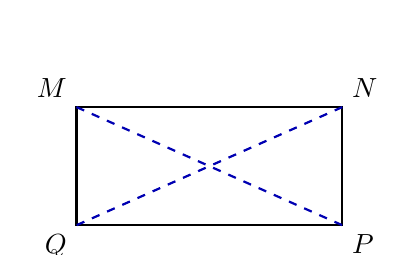
\begin{tikzpicture}[scale=0.75, baseline=(current bounding box.center)]
  \coordinate (M) at (0,2);
  \coordinate (N) at (4.5,2);
  \coordinate (P) at (4.5,0);
  \coordinate (Q) at (0,0);
  \draw[thick] (M) -- (N) -- (P) -- (Q) -- cycle;
  \draw[thick, dashed, blue!70!black] (M) -- (P);
  \draw[thick, dashed, blue!70!black] (N) -- (Q);
  \node[above left] at (M) {$M$};
  \node[above right] at (N) {$N$};
  \node[below right] at (P) {$P$};
  \node[below left] at (Q) {$Q$};
\end{tikzpicture}
\end{center}
\choice
{$MN$ và $QP$}
{\True $MP$ và $NQ$}
{$MQ$ và $NP$}
{$MN$ và $MQ$}
\loigiai{
Trong hình chữ nhật $MNPQ$, hai đường chéo nối các cặp đỉnh đối diện là $MP$ và $NQ$.
}
\end{ex}

\begin{ex}
Trong phép chia một số tự nhiên cho 4, số dư có thể là:
\choice
{1; 2; 3}
{0; 1; 2; 3; 4}
{\True 0; 1; 2; 3}
{0}
\loigiai{
Số dư trong phép chia một số tự nhiên cho 4 luôn nhỏ hơn 4 và lớn hơn hoặc bằng 0, tức là có thể nhận các giá trị $0; 1; 2; 3$.
}
\end{ex}

\begin{ex}
Số nào sau đây chia hết cho cả 2 và 5?
\choice
{\True 1150}
{1155}
{5311}
{3536}
\loigiai{
Số chia hết cho cả 2 và 5 phải có chữ số tận cùng là 0. Do đó trong các số đã cho, số 1150 chia hết cho cả 2 và 5.
}
\end{ex}

\begin{ex}
Hình nào trong các hình sau có hai cạnh đối song song và hai đường chéo bằng nhau?
\choice
{Hình bình hành}
{\True Hình thang cân}
{Hình thoi}
{Hình tam giác đều}
\loigiai{
Theo tính chất, hình thang cân có hai đáy (hai cạnh đối) song song với nhau và hai đường chéo bằng nhau.
}
\end{ex}

\begin{ex}
Cho tập hợp $A = \{0; 2; 4; a; b\}$. Khẳng định nào dưới đây là sai?
\choice
{\True $5 \in A$}
{$a \in A$}
{$0 \in A$}
{$1 \notin A$}
\loigiai{
Các phần tử thuộc tập hợp $A$ là $0, 2, 4, a, b$. Số 5 không có trong tập hợp $A$ ($5 \notin A$), do đó khẳng định "$5 \in A$" là sai.
}
\end{ex}

\begin{ex}
Số nào sau đây là ước của 60?
\choice
{16}
{18}
{\True 20}
{22}
\loigiai{
Thực hiện phép chia 60 cho các số đã cho: $60 : 20 = 3$ (chia hết). Vậy 20 là ước của 60.
}
\end{ex}

\begin{ex}
Trong các số sau, số nào là bội của 4?
\choice
{1}
{2}
{\True 8}
{15}
\loigiai{
Bội của 4 là các số chia hết cho 4. Trong các số trên, số 8 chia hết cho 4 ($8 : 4 = 2$).
}
\end{ex}

\begin{ex}
Trong các hình ảnh dưới đây, hình ảnh nào có dạng hình tam giác đều?
\begin{center}
\includegraphics[width=0.88\linewidth]{crops/test_p54_xref3332.jpeg}
\end{center}
\choice
{Hình 1}
{Hình 2}
{Hình 3}
{\True Hình 4}
\loigiai{
Hình 4 là chiếc đồng hồ treo tường dạng hình tam giác đều có 3 cạnh bằng nhau và 3 góc bằng nhau.
}
\end{ex}

\begin{ex}
Khẳng định nào sau đây là khẳng định đúng về hình chữ nhật?
\choice
{Bốn cạnh bằng nhau}
{\True Hai đường chéo bằng nhau và cắt nhau tại trung điểm mỗi đường}
{Hai đường chéo vuông góc với nhau}
{Chu vi hình chữ nhật là tích của chiều dài và chiều rộng}
\loigiai{
Theo tính chất của hình chữ nhật: hai đường chéo bằng nhau và cắt nhau tại trung điểm của mỗi đường.
}
\end{ex}

\begin{ex}
Cho $x$ là số tự nhiên thỏa mãn $10^7 < x < 10^8$. Số $x$ có:
\choice
{9 chữ số}
{\True 8 chữ số}
{7 chữ số}
{10 chữ số}
\loigiai{
Ta có $10^7 = 10\,000\,000$ (số nhỏ nhất có 8 chữ số) và $10^8 = 100\,000\,000$ (số nhỏ nhất có 9 chữ số).
Các số tự nhiên $x$ thỏa mãn $10^7 < x < 10^8$ là từ $10\,000\,001$ đến $99\,999\,999$, đều là các số có 8 chữ số.
}
\end{ex}

\begin{ex}
Hình chữ nhật có chiều dài $60\text{ dm}$ và chiều rộng $4\text{ m}$ thì diện tích là:
\choice
{\True $24\text{ m}^2$}
{$240\text{ dm}^2$}
{$200\text{ dm}^2$}
{$128\text{ dm}^2$}
\loigiai{
Đổi chiều dài về mét: $60\text{ dm} = 6\text{ m}$.
Diện tích hình chữ nhật là: $S = 6 \times 4 = 24\text{ (m}^2\text{)}$.
}
\end{ex}


\setcounter{ex}{0}
\noindent\textbf{\large PHẦN II. CÂU TRẮC NGHIỆM ĐÚNG SAI}
\vspace{1mm}
\begin{ex}
Cho các hình sau: hình tam giác đều, hình vuông, hình lục giác đều, hình chữ nhật, hình thoi, hình bình hành, hình thang cân. Xét tính đúng sai của các mệnh đề sau:
\choiceTF
{\True Hình tam giác đều, hình vuông, hình lục giác đều có tất cả các cạnh bằng nhau}
{\True Có 2 hình có hai đường chéo vuông góc với nhau}
{\True Có 3 hình hai cạnh đối song song và các đường chéo bằng nhau}
{Hình lục giác có độ dài đường chéo gấp đôi độ dài cạnh}
\loigiai{
\textbf{a)} Đúng. Tam giác đều có 3 cạnh bằng nhau, hình vuông có 4 cạnh bằng nhau và hình lục giác đều có 6 cạnh bằng nhau.

\textbf{b)} Đúng. Hai hình có hai đường chéo vuông góc với nhau là hình vuông và hình thoi.

\textbf{c)} Đúng. Ba hình có hai cạnh đối song song và các đường chéo bằng nhau là hình vuông, hình chữ nhật và hình thang cân.

\textbf{d)} Sai. Chỉ các đường chéo chính của hình lục giác đều mới có độ dài gấp đôi độ dài cạnh; các đường chéo phụ không có tính chất này và hình lục giác bất kỳ cũng không có tính chất này.
}
\end{ex}

\begin{ex}
Cho ba số $A = 24$, $B = 36$ và $C = 60$. Xét tính đúng sai của các mệnh đề sau:
\choiceTF
{\True Số 12 là một ước chung của ba số $A, B, C$}
{\True Phân tích số 24 ra thừa số nguyên tố ta được $2^3 \cdot 3$}
{Ước chung lớn nhất của hai số $A$ và $B$ là 6}
{\True Bội chung nhỏ nhất của hai số $A$ và $B$ là 72}
\loigiai{
\textbf{a)} Đúng. Cả ba số 24, 36 và 60 đều chia hết cho 12.

\textbf{b)} Đúng. Ta có $24 = 8 \cdot 3 = 2^3 \cdot 3$, trong đó 2 và 3 là các số nguyên tố.

\textbf{c)} Sai. Vì $24 = 2^3 \cdot 3$ và $36 = 2^2 \cdot 3^2$ nên $\text{ƯCLN}(24, 36) = 2^2 \cdot 3 = 12$.

\textbf{d)} Đúng. $\text{BCNN}(24, 36) = 2^3 \cdot 3^2 = 8 \cdot 9 = 72$.
}
\end{ex}


\setcounter{ex}{0}
\noindent\textbf{\large PHẦN III. CÂU HỎI TRẢ LỜI NGẮN}
\vspace{1mm}
\begin{ex}
Cho hình thoi $ABCD$ có cạnh $5\text{ cm}$. Chu vi của hình thoi $ABCD$ là bao nhiêu centimét? \shortans{20}
\loigiai{
Chu vi hình thoi $ABCD$ là: $5 \times 4 = 20\text{ (cm)}$. Đáp số: 20.
}
\end{ex}

\begin{ex}
Tìm số tự nhiên $x$ lớn nhất thỏa mãn $30 \ \vdots \ x$ và $45 \ \vdots \ x$? \shortans{15}
\loigiai{
Vì $x$ là số tự nhiên lớn nhất thỏa mãn $30 \ \vdots \ x$ và $45 \ \vdots \ x$ nên $x = \text{ƯCLN}(30, 45)$.
Ta có: $30 = 2 \cdot 3 \cdot 5$ và $45 = 3^2 \cdot 5$.
Do đó: $x = \text{ƯCLN}(30, 45) = 3 \cdot 5 = 15$. Đáp số: 15.
}
\end{ex}


\setcounter{ex}{0}
\noindent\textbf{\large PHẦN IV. TỰ LUẬN (HƯỚNG DẪN GIẢI VÀ THANG ĐIỂM)}
\vspace{1mm}
\begin{ex} (2,0 điểm)
Thực hiện phép tính (tính nhanh nếu có):
\begin{enumerate}[label=\textbf{\alph*)}, leftmargin=0.8cm, itemsep=2pt]
\item (0,5 điểm) $115 + 300 + 585$
\item (0,5 điểm) $6^2 \cdot 25 + 4 \cdot 9 \cdot 75 - 25^0$
\item (0,5 điểm) $2025 \cdot 79 + 2025 \cdot 21$
\item (0,5 điểm) $10^2 - [60 : (5^6 : 5^4 - 3 \cdot 5)]$
\end{enumerate}
\loigiai{
\textbf{a)} \textit (0,5 điểm): $\begin{aligned}[t] 115 + 300 + 585 &= (115 + 585) + 300 \\ &= 700 + 300 = 1000. \end{aligned}$

\textbf{b)} \textit (0,5 điểm): $\begin{aligned}[t] 6^2 \cdot 25 + 4 \cdot 9 \cdot 75 - 25^0 &= 36 \cdot 25 + 36 \cdot 75 - 1 \\ &= 36 \cdot (25 + 75) - 1 \\ &= 36 \cdot 100 - 1 = 3600 - 1 = 3599. \end{aligned}$

\textbf{c)} \textit (0,5 điểm): $\begin{aligned}[t] 2025 \cdot 79 + 2025 \cdot 21 &= 2025 \cdot (79 + 21) \\ &= 2025 \cdot 100 = 202500. \end{aligned}$

\textbf{d)} \textit (0,5 điểm): $\begin{aligned}[t] 10^2 - [60 : (5^6 : 5^4 - 3 \cdot 5)] &= 100 - [60 : (5^2 - 15)] \\ &= 100 - [60 : (25 - 15)] \\ &= 100 - [60 : 10] = 100 - 6 = 94. \end{aligned}$


}
\end{ex}
\vspace{1.5mm}

\begin{ex} (1,5 điểm)
Tìm số tự nhiên $x$, biết:
\begin{enumerate}[label=\textbf{\alph*)}, leftmargin=0.8cm, itemsep=2pt]
\item (0,25 điểm) $x + 24 = 60$
\item (0,25 điểm) $3(x - 5) = 21$
\item (0,5 điểm) $3 \cdot 2^x + 12 = 36$
\item (0,5 điểm) $150 - 2(x + 1) = 70$
\end{enumerate}
\loigiai{
\textbf{a)} \textit (0,25 điểm): $x = 60 - 24 \Rightarrow x = 36$.

\textbf{b)} \textit (0,25 điểm): $x - 5 = 21 : 3 \Rightarrow x - 5 = 7 \Rightarrow x = 7 + 5 \Rightarrow x = 12$.

\textbf{c)} \textit (0,5 điểm): $\begin{aligned}[t] 3 \cdot 2^x &= 36 - 12 \\ 3 \cdot 2^x &= 24 \\ 2^x &= 24 : 3 = 8 \\ 2^x &= 2^3 \\ x &= 3. \end{aligned}$

\textbf{d)} \textit (0,5 điểm): $\begin{aligned}[t] 2(x + 1) &= 150 - 70 = 80 \\ x + 1 &= 80 : 2 = 40 \\ x &= 40 - 1 = 39. \end{aligned}$


}
\end{ex}
\vspace{1.5mm}

\begin{ex} (1,0 điểm)
Bạn An đi nhà sách mua 5 cây bút bi cùng loại và 6 quyển tập cùng loại. Biết giá tiền một quyển tập là $10\,000$ đồng. Bạn đưa chị thu ngân tờ $200\,000$ đồng và được chị trả lại $125\,000$ đồng. Hỏi giá tiền của 1 cây bút mà bạn An đã mua là bao nhiêu?
\begin{enumerate}[label=\textbf{\alph*)}, leftmargin=0.8cm, itemsep=2pt]
\item (1,0 điểm) Tính giá tiền của 1 cây bút bi.
\end{enumerate}
\loigiai{
\textbf{a)} \textit (1,0 điểm): Tổng số tiền An đã dùng để mua bút và tập là:
$$200\,000 - 125\,000 = 75\,000\text{ (đồng).}$$
Số tiền An mua 6 quyển tập là:
$$6 \times 10\,000 = 60\,000\text{ (đồng).}$$
Số tiền An mua 5 cây bút bi là:
$$75\,000 - 60\,000 = 15\,000\text{ (đồng).}$$
Giá tiền của 1 cây bút bi mà bạn An đã mua là:
$$15\,000 : 5 = 3\,000\text{ (đồng).}$$
Đáp số: $3\,000$ đồng.


}
\end{ex}
\vspace{1.5mm}

\begin{ex} (0,5 điểm)
Cho $S = 3 + 3^2 + 3^3 + 3^4 + \dots + 3^{99} + 3^{100}$. Hỏi $S$ có chia hết cho 12 không? Vì sao?
\begin{enumerate}[label=\textbf{\alph*)}, leftmargin=0.8cm, itemsep=2pt]
\item (0,5 điểm) Chứng minh $S \ \vdots \ 12$.
\end{enumerate}
\loigiai{
\textbf{a)} \textit (0,5 điểm): Tổng $S$ có tất cả 100 số hạng. Vì $100 \ \vdots \ 2$, ta nhóm 2 số hạng liên tiếp thành một cặp như sau:
$$\begin{aligned} S &= (3 + 3^2) + (3^3 + 3^4) + \dots + (3^{99} + 3^{100}) \\ &= (3 + 9) + 3^2(3 + 3^2) + \dots + 3^{98}(3 + 3^2) \\ &= 12 + 3^2 \cdot 12 + \dots + 3^{98} \cdot 12 \\ &= 12 \cdot (1 + 3^2 + \dots + 3^{98}). \end{aligned}$$
Vì $12 \ \vdots \ 12$ nên tích $12 \cdot (1 + 3^2 + \dots + 3^{98})$ chia hết cho 12.
Vậy tổng $S$ có chia hết cho 12.


}
\end{ex}
\vspace{1.5mm}


\begin{center}
\rule{4cm}{0.4pt}\\
\textit{--- HẾT ---}
\end{center}
\end{document}
